\documentclass[a4paper,10pt]{article}
\usepackage[a4paper, total={167mm, 245mm}]{geometry}

\usepackage[colorlinks,linkcolor=blue,bookmarks,bookmarksopen,pdfauthor=krom]{hyperref}

\usepackage{fontspec}
\setmainfont[Path = fonts/, Extension = .ttf, BoldFont = ipagp]{ipamp}

\usepackage[normalem]{ulem}
\renewcommand{\ULthickness}{0.08em}

\usepackage[compact]{titlesec}
\titlespacing{\section}{0em}{*0}{*0}
\titlespacing{\subsection}{0em}{*0}{*0}
\titleformat{\section}{\normalfont\large}{\thesection}{0em}{}
\titleformat{\subsection}{\normalfont\large}{\thesection}{0em}{}

\setlength\parindent{1em}
\setlength\parskip{0em}
\renewcommand{\baselinestretch}{1.4}

\usepackage{fancyhdr}
\pagestyle{fancy}
\fancyhf{}
\renewcommand\headrulewidth{0pt}

\usepackage{graphicx}
\graphicspath{{images/}}

\begin{document}

\fancyfoot[R]{\thepage}

\small
\noindent\vspace{-2.2em}\begin{flushright}
2016/3/26 Revision
\end{flushright}

\vspace{62mm}

\LARGE
\textbf{\hskip 30mm OpenToonz}\par
\textbf{\hskip 30mm Startup Manual}\par
\Large
\textbf{\hskip 30mm InknPaint}

\noindent\begin{picture}(0,0)
\put(1,14){
\includegraphics[width=30mm]{OpenToonzLogo}}
\end{picture}

\newpage

\Huge
\noindent \textbf{Contents}\\[-0.7em]
\par
\Large
\noindent \textbf{\uline{\hskip -6em \hskip 6em Introduction\hskip 9.1em}}\\[0.4em]
\footnotesize
\setlength{\tabcolsep}{0em}
\renewcommand{\arraystretch}{1.15}
\begin{tabular}{p{22.2em}l}
\small ■ \footnotesize OpenToonz Main File Formats & p.3\\
\small ■ \footnotesize OpenToonz Interface & p.3\\
\small □ \footnotesize Room Information & p.3\\
\small □ \footnotesize Panel Customization & p.3\\
\small □ \footnotesize File Browser Interface & p.4\\
\end{tabular}\\[1.9em]

\par
\Large
\noindent \textbf{\uline{\hskip -6em \hskip 6em Scanning\hskip 10.6em}}\\[0.4em]
\footnotesize
\small □ \footnotesize GTS Scanning Tool \ \ \small ※ \footnotesize Please refer to the “GTS Manual".\\[1.9em]
\par
\Large
\noindent \textbf{\uline{\hskip -6em \hskip 6em Trace \large (Cleanup)\hskip 9.8em}}\\[0.4em]
\footnotesize
\setlength{\tabcolsep}{0em}
\renewcommand{\arraystretch}{1.15}
\begin{tabular}{p{22.2em}l}
\small □ \footnotesize tlv File Creation & p.4\\
\multicolumn{2}{l}{\small □ \footnotesize Without Antialiasing, Creating a tlv File With No Changes To Size \ \ \ \ \ p.8}\\
\end{tabular}\\[3.6em]

\par
\Large
\noindent \textbf{\uline{\hskip -6em \hskip 6em Finishing \large (InknPaint)\hskip 7.5em}}\\[0.4em]
\footnotesize
\setlength{\tabcolsep}{0em}
\renewcommand{\arraystretch}{1.15}
\begin{tabular}{p{22.2em}p{8.0em}p{22.2em}l}
\small □ \footnotesize Level File Loading & p.9 & \small □ \footnotesize Canceling an Operation & p.15\\
\small □ \footnotesize Level File Saving & p.9 & \small □ \footnotesize Displaying Sequential Frame Numbers & p.16\\
\small □ \footnotesize Level File Creation & p.9 & \small □ \footnotesize Duplication \& Deletion of the Frame & p.16\\
\small □ \footnotesize Palette File Saving & p.9 & \small □ \footnotesize Switching Image on the Display Menu & p.16\\
\small □ \footnotesize Scene File Loading & p.10 & \small □ \footnotesize Displaying Various Kinds of Window & p.17\\
\small □ \footnotesize Scene File Saving & p.10 & \small □ \footnotesize Palette Style Editing & p.17\\
\small □ \footnotesize Scene File Creation \& Closing a Scene File & p.10 & \small □ \footnotesize Studio Palette Information & p.18\\
\small □ \footnotesize OpenToonz Exiting & p.10 & \small □ \footnotesize Studio Palette Folder Creation \& Deletion, &\\
\small □ \footnotesize Cell Synthesis \& Cutting of Cells & p.11 & \hskip 1.5em to Create a New Palette. & p.18\\
\small □ \footnotesize Extracting Color from the Picture & p.13 & \small □ \footnotesize Viewing the Image & p.20\\
\small □ \footnotesize Connecting Broken Lines Automatically & p.13 & \small □ \footnotesize Time Sheet Editing & p.21\\
\small □ \footnotesize Line Modification & p.13 & \small □ \footnotesize Viewing the Color Swatch Used in Painting & p.21\\
\small □ \footnotesize Filling an Area & p.13 & \small □ \footnotesize Browsing the Files & p.22\\
\small □ \footnotesize Drawing with a Brush & p.13 & \small □ \footnotesize tlv Frame Viewing & p.22\\
\small □ \footnotesize Entering Text Characters & p.14 & \small □ \footnotesize Previewing Image Sequences in a Video & p.23\\
\small □ \footnotesize Turning Off the Line-Painted Area & p.14 & \multicolumn{2}{l}{\small □ \footnotesize Environment Settings \& Keyboard Shortcuts \ \ \ \ \ \ p.14}\\
\multicolumn{2}{l}{\small □ \footnotesize Image Copy/Paste Selected Range, \& Movement \ \ \ p.14} & \small □ \footnotesize Various Display Menus & p.23\\
\small □ \footnotesize Vector Image Editing & p.15 & \small □ \footnotesize Window Layout Customization & p.23\\
\small □ \footnotesize Image Display Tools & p.15 & \small □ \footnotesize tlv File Conversion to Other File Formats & p.24\\
\end{tabular}\\[1.9em]

\par
\Large
\noindent \textbf{\uline{\hskip -6em \hskip 6em Color Specification \large (PltEdit)\hskip 3.3em}}\\[0.4em]
\footnotesize
\setlength{\tabcolsep}{0em}
\renewcommand{\arraystretch}{1.15}
\begin{tabular}{p{22.2em}l}
\multicolumn{2}{l}{\small □ \footnotesize Sheet Creation to Perform Color Designation \ \ \ \ \ \ \ \ \ p.25}\\
\small □ \footnotesize Displaying a Specific Frame & \footnotesize p.25\\
\small □ \footnotesize Previewing in a Transparent Display & \footnotesize p.26\\
\end{tabular}

\fancyfoot[R]{\thepage
\begin{picture}(0,0)
\put(-523,-50){
\includegraphics[width=58em]{OpenToonzFooter}}
\end{picture}
}

\newpage

\phantomsection
\section*{\uline{■ OpenToonz Main File Formats}}
\addcontentsline{toc}{section}{■ OpenToonz Main File Formats}

\vspace{0.5em}
\normalsize
\ \ tnz: Xsheet File\par
\ \ tlv: Image File\par
\ \ tpl: Palette File\par
\ \ hst: History File\par
\ \ cln: Cleanup Configuration File\par
\ \ tif: GTS Scanned Image File\\
\\[-1em]
\small
※ tlv will display as an image sequence in Toonz, but is treated as a single file on the Windows browser.\\
Roughly speaking, in Toonz you configure the files inside the Scene \& Level.\\
Scene = 1 Cut Unit\\
Level = 1 Cell Unit\\

\phantomsection
\section*{\uline{■ OpenToonz Interface}}
\addcontentsline{toc}{section}{■ OpenToonz Interface}

\noindent OpenToonz's interface, contains something called a Room (Workspace) which is\\
used to place \& display panels for each software function.\\[-3.8em]

\phantomsection
\subsection*{\hskip 23.5em □ Room Information}
\addcontentsline{toc}{subsection}{□ Room Information}

\footnotesize
\hskip 34em Room shows menus \& layouts specific to each job\par
\hskip 34em by switching a tab (Top Right Corner of the Screen).\\
\par
\hskip 34em [Cleanup]: tif Image Conversion to tlv Image File\par
\hskip 34em [Pltedit]: BG (Background) Material \& tlv Colors\par
\hskip 34em [InknPaint]: tlv Line Refinement \& Coloring\par
\hskip 34em [Xsheet]: Synthesizes a Picture from a Time Sheet\par
\hskip 34em [Batches]: Performs Processing on Multiple Frames\par
\hskip 34em [Browser]: Used for Displaying \& Editing Files

\large
\noindent\begin{picture}(0,0)
\put(-10,-190){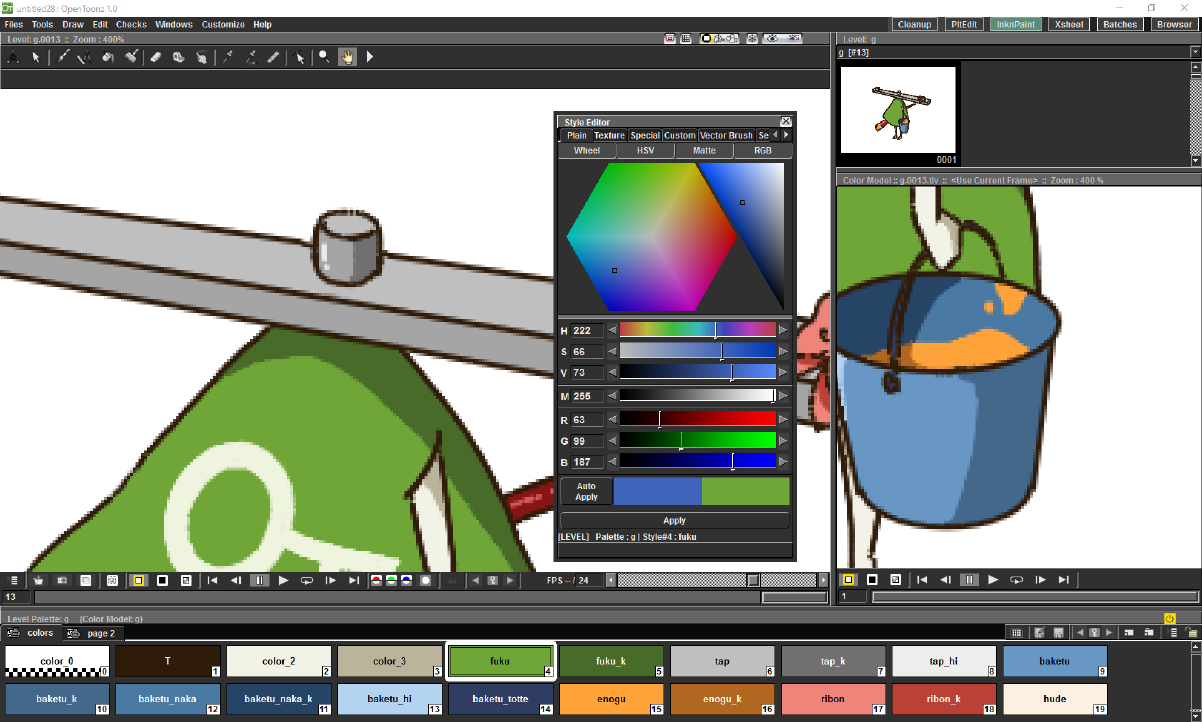
\includegraphics[width=28em]{OpenToonzInterfaceRoomPanels}}
\linethickness{0.1em}
\color{red}
\put(273,136){\line(1,0){122}}
\put(273,136){\line(-1,-5){26}}
\put(139,-222){\line(-1,0){142}}
\put(139,-222){\line(1,2){43}}
\end{picture}\\[15em]

\phantomsection
\subsection*{□ Panel Customization}
\addcontentsline{toc}{subsection}{□ Panel Customization}

\footnotesize
\noindent ・Individual panels will be displayed by selecting them from the [Windows] menu.\\
・Each panel can be docked into the Room. Display the guide of the position to be docked by dragging \& moving the\\
title bar of each panel, when you release the mouse button it will switch to the new docking layout.\\
・If you want to return the docked panel to a floating window, uncheck the [Customize > Lock Room Panes], \& take it out\\
of the docked position by dragging on the title bar part.\\
・If you do not want to release any fixed windows by mistake, make sure to check the [Customize > Lock Room Panes].

\newpage

\phantomsection
\subsection*{\uline{□ File Browser Interface}}
\addcontentsline{toc}{subsection}{□ File Browser Interface}

\small
\noindent File Browser, is a panel to carry out work on files, such as saving \& loading.\\
A tree structure is displayed on the left side of the folder, with the contents on the right-hand side.

\large
\noindent\begin{picture}(0,0)
\put(108,-165){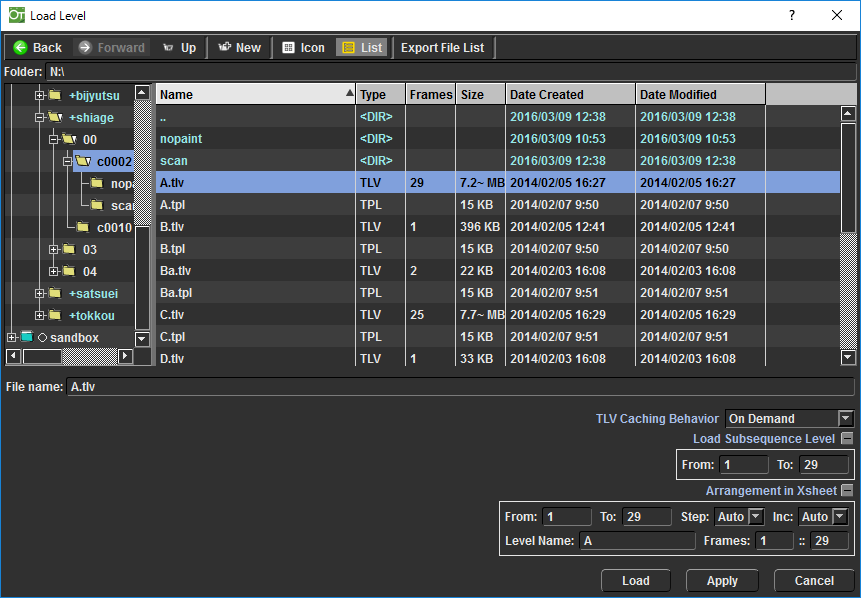
\includegraphics[width=21.2em]{OpenToonzInterfaceFileBrowserInterface}}
\end{picture}\\[12em]

\phantomsection
\section*{\uline{■ Cleanup (Trace)}}
\addcontentsline{toc}{section}{■ Cleanup (Trace)}

\small
\noindent In the Cleanup process, use the scanned tif format file that you created using the GTS* scanning tool,\\
to create a paint file (Toonz Raster Level File: tlv).\\
※ Please refer to the “GTS Manual" for information about scanning using GTS.\\
Switch to the Cleanup Room when doing this work.\\
tlv image size, position to be cut, density of lines, \& output destination settings, can be performed.\\

\phantomsection
\subsection*{\uline{□ tlv File Creation}}
\addcontentsline{toc}{subsection}{□ tlv File Creation}

\small
\noindent 1. Load the tif file scanned by GTS into the Xsheet.

\large
\noindent\begin{picture}(0,0)
\put(116,-115){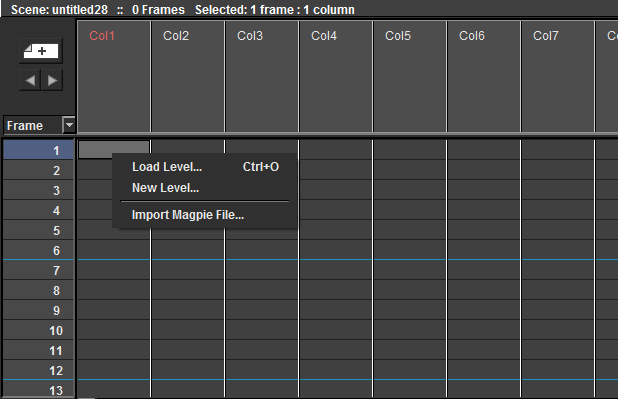
\includegraphics[width=20em,height=10.5em]{CleanupTLVFileCreationTIFImport}}
\end{picture}\\[8.2em]

\footnotesize
\noindent In Xsheet, select the Column you want to place the tif, select Load Level using right-click on Column Frame or File Menu.\\
※ If you have created a Configuration File (cln), you can select the tif file, using the Cleanup Settings Window [Load]\\
\& Load the configuration file. The Load result will be reflected in the value of the Cleanup Settings.\\
\\
\small
2. Select the tif file you want to preview.\\
\footnotesize
Layout sorting → will continue to work in the current order, the main viewer will show the Cell → other Cells.\\
If an image overlaps the tif you wanted to preview, display only the required picture with [Camera Stand Visibility Toggle].\\
\\
\small
\uline{※ If manually setting the size goto step 3. If doing work by reading a settings file goto Step 5.}\\
\\
3. If the angle of the tif image is tilted it will need to be fixed to the correct angle.\\
\footnotesize
[Rotate]: Select angle with the Cleanup Camera Test Preview, Rotate value will be reflected in the clockwise direction.\\
\ [Flip]: It can flip the picture Left \& Right, or Up \& Down.

\newpage

\small
\noindent 4. Camera Test Cleanup for setting the size.\\
\footnotesize
Select [Processing/Camera Test]. The Red Frame represents the Range to be cut from the tif image displayed on the Viewer.\\
□ Click \& Drag on the Red Frame Range edges to scale, Click \& Drag on the Red Frame Range center cross to move.\\
Cleanup will retain the current DPI after stretching the Canvas Size. Resolution (Pixel Size) will be changed to fit\\
the new Canvas Size.\\
\ [Forced Squared Pixel]: When turned ON, the aspect ratio of pixels is forced to 1:1.

\large
\noindent\begin{picture}(0,0)
\put(108,-144){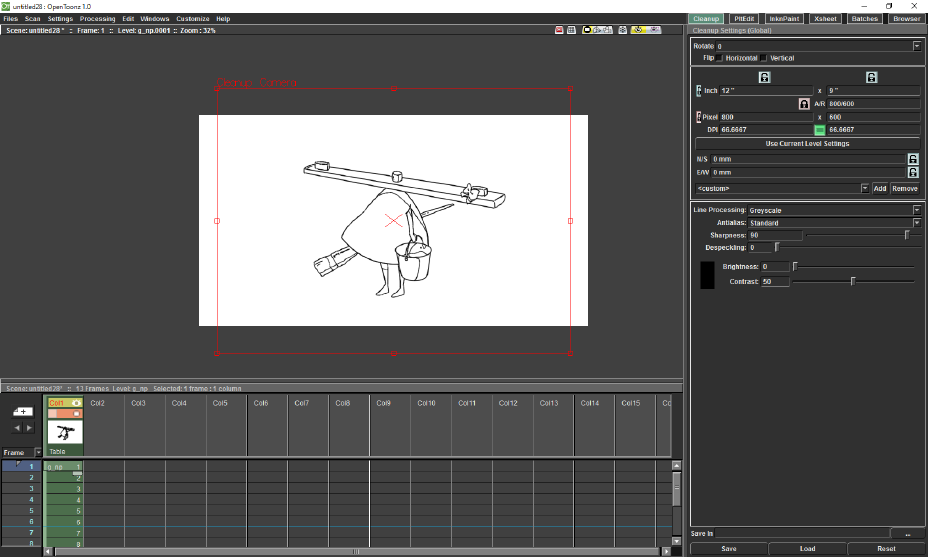
\includegraphics[width=21.7em]{CleanupTLVFileCreationCameraTest}}
\end{picture}\\[11em]

\small
\noindent 5. Preview.\\
\footnotesize
Select [Processing/Preview Cleanup].\\
\\
\small
6. For previewing the image, processing line thickness, \& adjusting the adaptive Antialiasing degree.\\
\footnotesize
If line processing is not required, set the Line Processing option to None. The Greyscale option is for if you want to\\
recognize the lines as shades of Grey, if you want to recognize them as colored choose the Color option instead.

\large
\noindent\begin{picture}(0,0)
\put(145,-197){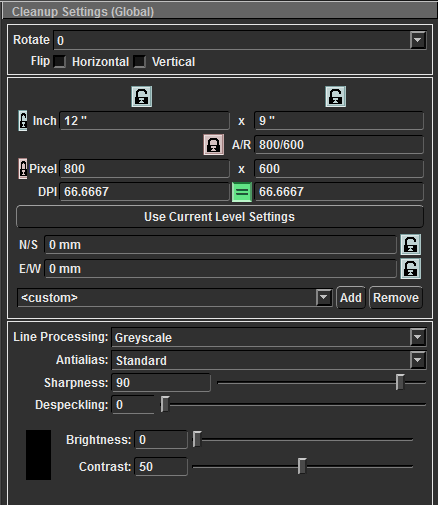
\includegraphics[width=15.3em]{CleanupTLVFileCreationCleanupSettings}}
\end{picture}\\[15em]

\footnotesize
\noindent Antialias Setting\\
\ [Standard]: It adds Antialiasing using the resampling process when changing the scale.\par
\hskip 4.3em For output DPI, is recommended to perform this process on images shortened to less than 90\% of the original size.\\
\ [None]: It does not perform Antialiasing.\\
\ [Morphological]: Uses smoothing by analyzing the edges of the image. There is no need to reduce the image size.\\
\ [Brightness]: The thickness of the line will be changed. The lower the value, the thicker the line will become.\\
\ [Contrast]: Adjusts the application degree of Antialiasing. A higher value makes the pixels more clear, a smaller value\\
will make the pixels more aliased.\\
The amount of Antialiasing can be checked by enabling the [Processing/Opacity Check].\\
※ Usually set to the same value as Brightness. When less than the Brightness, all of the lines will be semi-transparent.\\
※ If you set None or Morphological on the Antialias setting, the Contrast parameter will have no effect.

\newpage

\noindent [Sharpness]: Used to define the sharpness degree of the lines. A higher value will generate hard Sharp lines.\\
With a low value, it will make the lines become more smooth.\\
\ [Despeckling]: Remove any small spots from the image. The value is the size of the maximum area to be removed, in pixels.\\
You can see the spots that will be removed by enabling the Opacity Check.\\
\ [MLAA Intensity]: Sets the blur strength in Morphological Antialiasing. Numeric value is how large the line blur is.\\
(Only available when Morphological Antialiasing is selected)\\
\\
\small
If using Color line drawing, adjust the parameters, to detect how each color in the image is divided.
\footnotesize
・Cleanup processing automatically sets the color assigned to the lines.\\
Colors to be used for recognition, colors are either assigned in post-recognition or by selecting Edit from the box at\\
the bottom of the Style Editor, you can change each color. ①  Inside the Color Box is a Color used in the recognition\\
② is also assigned. It is also possible to pick color values from an image in the work area using the RGB Picker tool.

\large
\noindent\begin{picture}(0,0)
\put(34,-233){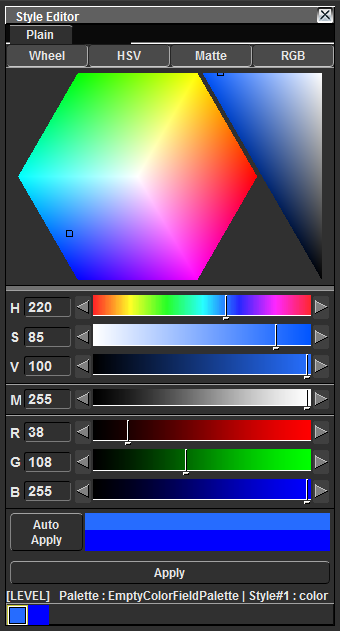
\includegraphics[width=11em]{CleanupTLVFileCreationStyleEditor}}
\put(228,-323.5){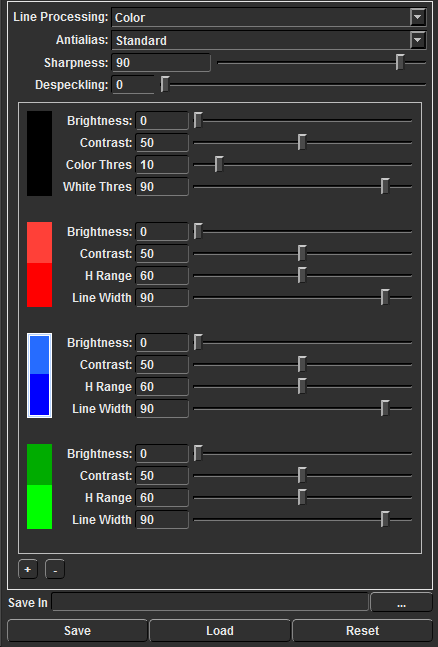
\includegraphics[width=18.9em]{CleanupTLVFileCreationLineProcessingColor}}
\put(206,-176.5){①}
\put(206,-196.5){②}
\put(34.5,-254){①}
\put(60,-254){②}
\linethickness{0.1em}
\color{red}
\put(216,-172){\line(1,0){29}}
\put(216,-192){\line(1,0){29}}
\put(37.5,-242){\line(0,1){13}}
\put(59,-242){\line(-1,1){13}}
\end{picture}\\[25.4em]

\footnotesize
\noindent ・If using black you can set different parameters. Black is usually defined when using solid lines in a line drawing.\\
Other colors are usually defined as color shaded lines, such as shadows \& highlights.\\
・Add or remove a color from the list by clicking the buttons [+][-] in the part under the Color List.\\
・Following is a list of parameters that can be set in the color list, in addition to the above parameters.\\
\ [Color Threshold]: The threshold amount of how much between the Black \& Color pixel recognition will be. The higher the\\
value, the higher the amount of pixels will be considered to be color.\\
\ [White Threshold]: The threshold of pixels to be considered as white. e.g. use it to ignore the color of the paper.\\
The higher the value, the higher the amount of pixels will be considered to be white.\\
\ [H Range]: Sets the color range for the color recognition. The higher the value, the higher the color range of pixels.\\
\ [Line Width]: Sets the width of the colored lines to be displayed. Lines will be thicker with a higher value.\\
\par
\small
\noindent 7. Specify output location of the tlv file [Save In] under the Cleanup Settings window, after Line Processing.\\

\newpage 

\noindent 8. [Save Settings] in [Cleanup Settings] will save the settings.\\
\footnotesize
Click the [Save] button under the Cleanup Settings window, when you have finished all the settings, \& save the Cleanup\\
configuration file by specifying the location (extension cln).\\
※ cln file, please save it in the same folder hierarchy as the original tif file that was used.\\
※ When you select a tif \& you have already created a cln, it will Load the cln values automatically.\\
Using the same name in the Level, saving in the same location, it can also be used on the Animation Level. In this case,\\
the settings are automatically displayed when you select the tlv, when using a tlv file Cleanup is always used.\\
Settings of the loaded cln in the project \& scene, will become the default settings.\\
\\
\small
9. If you want to Cleanup the next cell, repeat steps 2-8.\\
\\
10. After you save the cln files of all of the cells, you can then save the entire Xsheet data.\\
\footnotesize
Once you have saved all of the cln files, save the Xsheet using [Files/Save Scene As].\\
\\
\small
11. Doing the Cleanup.\\
\footnotesize
\uline{【If you want to cleanup all the tif files in the cut】}\\
Select [Windows/Other Windows/Tasks], to display the Tasks window.\\
In the dialog that appears when you click the Tasks menu [Add Cleanup] button, select the tnz file that you want to\\
cleanup, \& then click OK.\\
Tasks menu registers the tnz files you select, select all the tasks that need to be registered.\\
\ When you click the [Start] button, the calculation will begin.\\
\\
The state of the calculation is confirmed by the [Status].\\
\ [Suspended]: Paused\\
\ [Running]: Calculating\\
\ [Completed]: Calculation has completed successfully\\
\\
\ When it is finished [Status] is [Completed], select Remove from the Tasks menu, to remove the registered tnz files.\\
\ [Files/New Scene] will update, read the tnz file again with [Load Scene], tif displays on Xsheet (Light Blue) tlv is (Green).\\
\par
\hskip 27.5em \uline{【If you want to cleanup only tif files selected in the Xsheet】}\par
\hskip 28em Select tif placed in Xsheet, if you select [Processing/Cleanup],\par
\hskip 28em the cleanup dialog box will appear.\\
\par
\hskip 28em ① The selected frame number is shown above the progress bar.\par
\hskip 28em ② Cleanup View ON/OFF\par
\hskip 28em ③ [Cleanup]: Only Cleanup 1 frame.\par
\hskip 28em \ \ \ [Skip]: Skip 1 frame in the Cleanup. (To move to the next\par
\hskip 28em frame, skipped frame is not executed.)\par
\hskip 28em \ \ \ [Cleanup All]: All the frames will Cleanup.\par
\hskip 28em \ \ \ [Cancel]: Cancel the Cleanup.

\large
\noindent\begin{picture}(0,0)
\put(16,-36){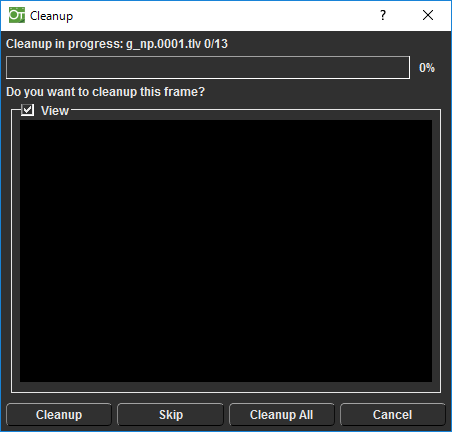
\includegraphics[width=17.3em]{CleanupTLVFileCreationCleanupFrame}}
\color{white}
\put(8,133){●}
\put(8,109){●}
\put(8,-33){●}
\color{red}
\put(8,133){①}
\put(8,109){②}
\put(8,-33){③}
\end{picture}\\[3em]

\small
\noindent 12. When you have finished the calculation of the Cleanup, make sure tlv files have been created properly.\\
\footnotesize
Select [Files/Load Scene] from the InknPaint Room, \& Load the tnz file that was calculated with Cleanup.\\
Select a tlv file on the Xsheet window \& select [Right-Click Menu/Info]. On Image Size, you can check the Dpi information.\\
To check the movement of animation frames, select a Cell in the Level Strip \& use [Edit/Next Frame (Previous Frame)].

\newpage 

\phantomsection
\subsection*{\uline{□ Without Antialiasing, Creating a tlv File With No Changes To Size}}
\addcontentsline{toc}{subsection}{□ Without Antialiasing, Creating a tlv File With No Changes To Size}

\small
\noindent In the file conversion function, you can also create a tlv from general-purpose image sequence files\\
such as tif \& tga. Right-click on the file you want to convert in the file browser, \& select Convert...

\large
\noindent\begin{picture}(0,0)
\put(3,-165){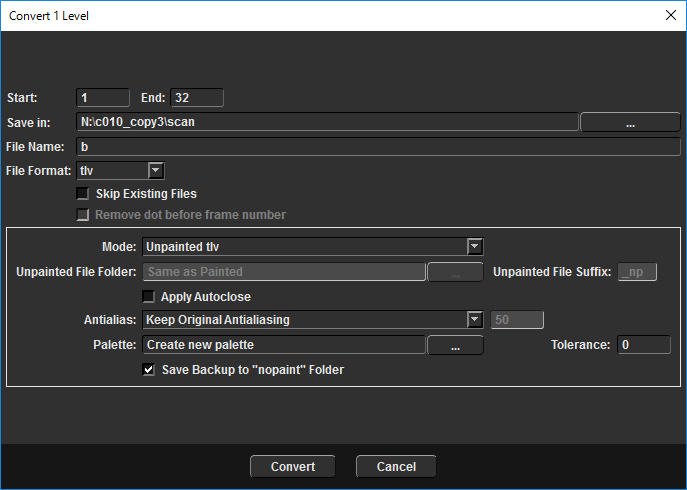
\includegraphics[width=19.2em]{WithoutAntialiasingConvert1Level}}
\color{white}
\put(19,-66.5){\small{●}}
\put(19,-76){\small{●}}
\put(28,-86){\small{●}}
\color{red}
\put(-6,-35){\footnotesize{①}}
\put(-6,-44){\footnotesize{②}}
\put(-6,-53){\footnotesize{③}}
\put(-6,-62){\footnotesize{④}}
\put(19,-66.5){\small{⑤}}
\put(19,-76){\small{⑥}}
\put(28,-86){\small{⑦}}
\end{picture}\\[12.6em]

\small
\noindent ① Enter the frame range that you want to create.\\
② Select the destination of where the created tlv files will be saved.\\
③ Enter the file name.\\
④ Select the file format. If you want to create tlv files, select the tlv option.\\
⑤ When checked, if there are already existing tlv files in the destination, it only creates new tlv files,\\
\& will not overwrite any existing files, skipping them.\\
⑥ When checked, it deletes the attached [.(Dot)] on the front of the frame number of the file name of tlv\\
before conversion. This function is used if you want to convert from a tlv file to tga \& other file formats.\\
※ The function is enabled, only if the file format after the conversion is not selected to be a tlv.\\
Refer to “tlv File Conversion to Other File Formats" (p.24) for more information.\\
⑦ If you want to convert from sequence image file of a \uline{Line Drawing} with no Antialiasing to a tlv select\\
\ [\uline{Unpainted} tlv from non AA source]. With no Antialiasing, if you want to convert from an \uline{Already Painted}\\
image sequence file to tlv select [\uline{Painted} tlv from non AA source]. When converting painted image files to\\
tlv, a one-pixel line to the boundary of the fill will be automatically added (appearance will not change).

\newpage

\phantomsection
\section*{\uline{■ InknPaint}}
\addcontentsline{toc}{section}{■ InknPaint}

\noindent InknPaint room is used primarily in the finishing process.\\[-0.3em]

\phantomsection
\subsection*{\uline{□ Level File Loading (Files/)}}
\addcontentsline{toc}{subsection}{□ Level File Loading (Files/)}

\normalsize
\noindent Load Level… Loads a tlv Level file, it will also load the\\
tpl Palette File that is attached to it.\\[1.6em]
Load Folder… Has the ability to specify a set range of\\
frames.\par
\footnotesize
\noindent From the Start-Frame, To the End-Frame.\\
When painting, \&  more than 1 person is working on a tlv file, enter only\\
the frame, which each user is working on in here.\\
(※ If you open the same frame, when you save the Level, all of the\\
frames that are open will be overwritten.)\\
\par
\normalsize
\noindent Arrangement in Xsheet…Load is used to specify the display\\
method of the Xsheet.\par
\footnotesize
\noindent From the Start-Frame, To the End-Frame.\\
Step can specify the number of frames for each frame.\\
Example) 1 is the input → 1,2,3‥ 2 is the input → 1,1,2,2,3,3‥\\
Inc can omit frames in the stepping sequence.\\
Example) 2 is the input → 1,3,5‥ 3 is the input → 1,4,7‥\\
The Xsheet displays only the number of frames specified in From, To, but\\
all of the frames are read inside the tlv file.

\large
\noindent\begin{picture}(0,0)
\put(295,29){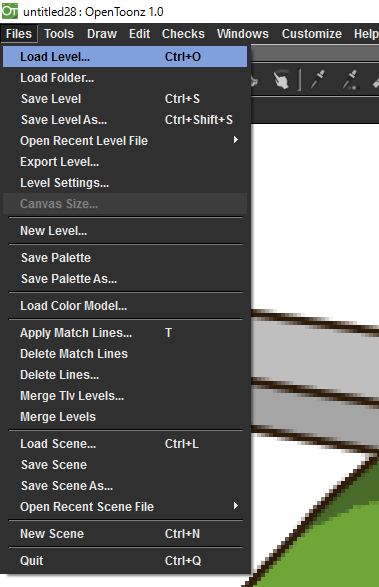
\includegraphics[width=14.8em]{InknPaintLevelFileLoading}}
\end{picture}\\[-2.7em]

\phantomsection
\subsection*{\uline{□ Level File Saving (Files/)}}
\addcontentsline{toc}{subsection}{□ Level File Saving (Files/)}

\normalsize
\noindent Save Level… Saves the currently selected tlv file.\par
\footnotesize
\noindent The following alert window will be displayed if you have not yet saved the tpl (Palette File) when running the save.\\
Overwrite Palette… tlv file will be saved, \& tpl file will be overwritten.\\
Don't Overwrite Palette… tlv file will be saved, \& tpl file will not be saved.\\[-0.7em]
\par
\normalsize
\noindent Save Level As… Saves the tlv files you are currently working on with a different name.\\
\footnotesize
The tpl that is attached to the tlv is also saved at the same time. (If you save A.tlv, A.tpl will also get saved)\\[-1em]
\\
\normalsize
Open Recent Level File… tlv files used recently are displayed in the History, select to Load a tlv.\\[-0.6em]
\\
Level Settings… Information about a currently selected tlv file will appear in a separate window.\\[-0.5em]

\phantomsection
\subsection*{\uline{□ Level File Creation (Files/)}}
\addcontentsline{toc}{subsection}{□ Level File Creation (Files/)}

\noindent New Level… Creates a new tlv Level file.\\[-0.7em]

\phantomsection
\subsection*{\uline{□ Palette File Saving (Files/)}}
\addcontentsline{toc}{subsection}{□ Palette File Saving (Files/)}

\noindent Save Palette… Saves the Palette File (tpl) of the currently selected tlv file.\par
\footnotesize
\noindent The following dialog appears when you select this menu.\\
Overwrite… tpl file will be saved\\
Don't Overwrite… tpl file will not be saved\\
※ Destination Path will appear.\\[-1.2em]
\par
\normalsize
\noindent Save Palette As… Saves the Palette File (tpl) of a currently selected tlv file as another name.

\newpage

\newpage

\phantomsection
\subsection*{\uline{□ Scene File Loading (Files/)}}
\addcontentsline{toc}{subsection}{□ Scene File Loading (Files/)}

\noindent Load Scene… Loads a tnz Scene file.\\[-0.7em]

\phantomsection
\subsection*{\uline{□ Scene File Saving (Files/)}}
\addcontentsline{toc}{subsection}{□ Scene File Saving (Files/)}

\noindent Save Scene… Saves the tnz Scene file.\\
\\
Save Scene As… Saves the tnz Scene file with an alias name.\\
\\
Open Recent Scene File… tnz files used recently are displayed in the History, select to Load a tnz.\\

\phantomsection
\subsection*{\uline{□ Scene File Creation \& Closing a Scene File (Files/)}}
\addcontentsline{toc}{subsection}{□ Scene File Creation \& Closing a Scene File (Files/)}

\noindent New Scene… Creates a new Scene (tnz) file. Also used when you close a currently opened file.\\
\footnotesize
If you do not save the Scene, you will be prompted to select whether to close without saving or overwrite the changes.\\
In order to close a Scene file that is currently open without saving, select [Discard].\\
If there is unsaved changes to a tlv Level file, a confirmation dialog box will appear.\\

\phantomsection
\subsection*{\uline{□ OpenToonz Exiting (Files/)}}
\addcontentsline{toc}{subsection}{□ OpenToonz Exiting (Files/)}

\normalsize
\noindent Quit… Exits the OpenToonz application.\\
\footnotesize
If you have not saved any data, you will be prompted to select whether to close without saving or overwrite the changes.

\newpage

\phantomsection
\subsection*{\uline{□ Cell Synthesis \& Cutting of Cells}}
\addcontentsline{toc}{subsection}{□ Cell Synthesis \& Cutting of Cells}

\small
\noindent In OpenToonz, by treating the Xsheet panel as a synthetic strip, you can carry out the synthesis of cells.\\
\ Run [Files/Apply Match Lines] to synthesize a line of 2 tlv Level files.\par
\normalsize
\noindent 【Step 1】\\
\footnotesize
In the Xsheet on the right side of the current tlv (Synthesis Parent. Match Line tlv), place the Match Line of the tlv\\
(Synthesis Child. Match Line tlv). Arrange together as best possible each cells frame number on the Xsheet to paste.\\
(※ The image below is the arrangement of the sheet in the case where you want to paste a line from F1 to G8~13)\par
\normalsize
\noindent 【Step 2】\\[-0.5em]
\par
\footnotesize
\noindent \hskip 27.5em ㋐ Current tlv (Synthesis Parent. Match Line tlv)\par
\noindent \hskip 27.5em ㋑ Match Line tlv (Synthesis Child. Match Line tlv)\\[-5em]

\noindent \hskip 27.5em ○\par
\noindent \hskip 27.5em ○

\large
\noindent\begin{picture}(0,0)
\put(82,-135){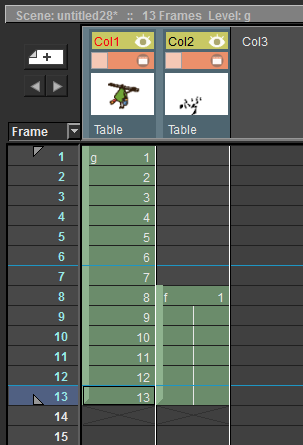
\includegraphics[width=10.7em]{InknPaintCellSynthesisCuttingXsheet}}
\color{white}
\put(128,32.5){\large{●}}
\put(159,32.5){\large{●}}
\color{red}
\put(128,32.5){\large{○}}
\put(159,32.5){\large{○}}
\put(128,32.5){\large{㋐}}
\put(159,32.5){\large{㋑}}
\end{picture}\\[9.5em]

\footnotesize
\noindent Select both of the columns, \& then select the Apply Match Lines menu.

\large
\noindent\begin{picture}(0,0)
\put(73,-215){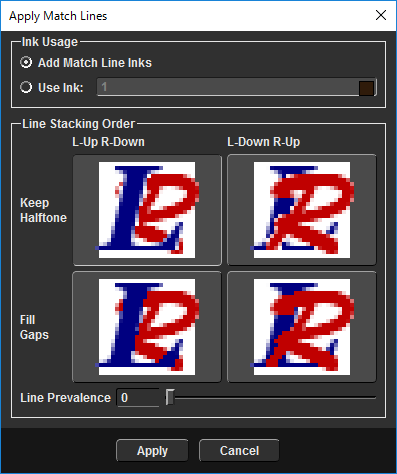
\includegraphics[width=15.2em]{InknPaintCellSynthesisCuttingApplyMatchLines}}
\put(307,-99){
\includegraphics[width=8.9em]{InknPaintCellSynthesisCuttingApplyMatchLinesLR}}
\color{white}
\put(70,-20){\normalsize{●}}
\put(70,-59){\normalsize{●}}
\put(344,-18.5){\large{●}}
\put(379,-24){\large{●}}
\color{red}
\put(70,-20){\normalsize{①}}
\put(70,-59){\normalsize{②}}
\put(344,-18.5){\large{○}}
\put(379,-24){\large{○}}
\put(344,-18.5){\large{㋐}}
\put(379,-24){\large{㋑}}
\end{picture}\\[15.5em]

\normalsize
\noindent 【Step 3】\\
\footnotesize
The following window is displayed. Using Match Lines, setup how much the line bleeds into the Ink, \& run to paste.\\
\small
① Ink Usage\par
\footnotesize
\noindent  [Add Match Line Inks]: Pastes in the Match Line colors using the lines in the tlv. The palette of the current working\\
page that [Match Lines] has created, will have copied across any new colors that have been used.\\
\ [Use Ink]: Specifies a style number from the current working Level, \& then pastes the tlv into that color.\\
\\
※ If you do not want to use all of the lines to paste, so any unnecessary lines can be deleted later, paste\\
to create a temporary style rather than the style you want to actually use.

\newpage

\footnotesize
\setlength{\arrayrulewidth}{0.1em}
\renewcommand{\arraystretch}{1}
\setlength{\tabcolsep}{0.3em}
\noindent \hskip 11em \begin{tabular}{|p{17.0em}|}
\hline
\small{L-Up R-Down・Keep Halftone}\\
\small{Line Prevalence [0]}\\
\scriptsize{・Uses the original image Antialiasing}\\[-0.3em]
\scriptsize{・Match Lines uses original Antialiasing}\\[-0.3em]
\scriptsize{Example) Cut lines (BG Cuts, Cell Cuts),}\\[-0.3em]
\scriptsize{pasting of missing videos, etc.}\\[1.5em]
\hline
\end{tabular}\\[-10.8em]

\noindent \hskip 41.7em \begin{tabular}{|p{19.0em}|}
\hline
\small{L-Down R-Up・Keep Halftone}\\
\small{Line Prevalence [100]}\\
\scriptsize{・Uses the original image Antialiasing}\\[-0.3em]
\scriptsize{・Match Lines uses original Antialiasing}\\[-0.3em]
\scriptsize{Example) Synthesis element solid line is}\\[-0.3em]
\scriptsize{drawn in shadow line \& combined with parent}\\[1.5em]
\hline
\end{tabular}\\[0.5em]

\noindent \hskip 11em \begin{tabular}{|p{17.0em}|}
\hline
\small{L-Up R-Down・Fill Gaps}\\
\small{Line Prevalence [30]}\\
\scriptsize{・Match Lines erodes the Antialiasing in}\\[-0.3em]
\scriptsize{the original image}\\[-0.3em]
\scriptsize{・Match Lines uses original Antialiasing}\\[-0.3em]
\scriptsize{Example) Pasting of synthesis images}\\[1.5em]
\hline
\end{tabular}\\[-10.8em]

\noindent \hskip 41.7em \begin{tabular}{|p{19.0em}|}
\hline
\small{L-Down R-Up・Fill Gaps}\\
\small{Line Prevalence [70]}\\
\scriptsize{・Uses the original image Antialiasing}\\[-0.3em]
\scriptsize{・Match Lines Antialiasing is eroded by the}\\[-0.3em]
\scriptsize{original image}\\[-0.3em]
\scriptsize{Example) Pasting of synthesis images}\\[1.5em]
\hline
\end{tabular}

\large
\noindent\begin{picture}(0,0)
\put(5,94.6){
\includegraphics[width=6.6em]{InknPaintLineStackingOrderLRKeepHalftone}}
\put(250,94.6){
\includegraphics[width=6.6em]{InknPaintLineStackingOrderRLKeepHalftone}}
\put(5,4.5){
\includegraphics[width=6.6em]{InknPaintLineStackingOrderLRFillGaps}}
\put(250,4.5){
\includegraphics[width=6.6em]{InknPaintLineStackingOrderRLFillGaps}}
\end{picture}\\[-1em]

\small
\noindent ② Line Stacking Order\\
\footnotesize
Match Lines sets the condition \& how much the paste will bleed into the Ink.\\
\ [Line Prevalence] can be set from 0 upto 100, 0 is Match Lines without affecting all the picture you are currently working\\
 on, 100 will stick Match Lines on top \& completely overlap the lines that are currently being worked on.\\
The 4 selection windows displayed above make it easier to understand the values commonly used in Line Prevalence.\\
Each of the values can be viewed on each window, upper-left [0], upper-right [100], lower-left [30], \& lower-right [70].\\[0.7em]
\par
\normalsize
\noindent 【Step 4】\\
\footnotesize
When Cutting lines, you can create a new style for the lines. The color of lines, is the re-paint style you have created.\\
In the case of synthetic paste \& re-fill of the line style is the color that you want to actually use in the line area.\\
※ If you do not want to include the Fill color of Cut lines, set the Matte value of the Cut lines style to 0.\\[0.7em]
\par
\normalsize
\noindent 【Step 5】\\
\small
\ [Files/Delete Match Lines] menu, can be used to erase the line style of the currently selected tlv.\\
\footnotesize
The following window is displayed when you select the menu.\\
\ [Style Index]: Specifies the style number to apply.\\
\ [Apply to Frames]: Specifies the frame number to be applied.\\
※ In case you want to specify consecutive frame numbers, connect them with a [- (Hyphen)].\\
Example) To erase frames from 3 to 18 → 3-18\\
※ If you want to specify the frame stepping, enter frames separated by a [, (Comma).\\
Example) To only erase frames 1, 3, 6 → 1,3,6

\newpage

\phantomsection
\subsection*{\uline{□ Extracting Color from the Picture (Tools/)}}
\addcontentsline{toc}{subsection}{□ Extracting Color from the Picture (Tools/)}

\large
\noindent\begin{picture}(0,0)
\put(0,0){
\includegraphics[width=1em]{ToolStylePicker}}
\end{picture}\\[-3.2em]

\normalsize
\noindent\hskip 1.3em Style Picker Tool… Used to pick data, extracts color \& style number by clicking on tlv area.
\par
\footnotesize
\noindent By clicking where you want to on the tlv display, palette \& styles are then linked. You can extract from Areas \& Lines\\
individually. A Shortcut key for the tool can also be assigned separately.\\[-0.3em]

\large
\noindent\begin{picture}(0,0)
\put(0,0){
\includegraphics[width=1em]{ToolRGBPicker}}
\end{picture}\\[-3.2em]

\normalsize
\noindent\hskip 1.3em RGB Picker Tool… Has the ability to extract any colors displayed in the Viewer (RGB Values).\par
\footnotesize
\noindent A Non-Normal selection, calculates the average RGB value in the range enclosed. Colors are reflected in the Style Editor.\\
When Passive Pick is checked, it will display in the toolbar the RGB value of the position of the cursor in real time.\\[-0.3em]

\phantomsection
\subsection*{\uline{□ Connecting Broken Lines Automatically (Tools/)}}
\addcontentsline{toc}{subsection}{□ Connecting Broken Lines Automatically (Tools/)}

\large
\noindent\begin{picture}(0,0)
\put(0,0){
\includegraphics[width=1em]{ToolTape}}
\end{picture}\\[-3.2em]

\normalsize
\noindent\hskip 1.3em Tape Tool… If there are breaks in the line drawing, it can automatically connect the lines.\par
\footnotesize
\noindent When you run it on a line portion that is interrupted to some extent, it connects the lines with a width of 1 pixel.\\
Switch the Type depending on the type of picture, you can use it to decide the numerical value.\\
\ [Type - Normal]: Click the line connections in the viewer. There is a possibility it may create unnecessary portions.\\
\ [Type - Rectangular, Freehand, Polyline]: Run the line connection only to the extent enclosed.\\
\ [Frame Range]: Run the Tape Tool on a plurality of frames.\\
\ [Distance]: Set the maximum number of pixels that are connected. Reference Value) 50\\
\ [Angle]: Set the maximum angle to be connected. Reference Value) 90\\
\ [Style Index]: Set color of connecting line. Enter style number, it can be changed by clicking on a style in the palette.\\
\ [Opacity]: Set the concentration of the lead line. And to 255 at the time of paint in a two-value with no anti-aliasing.\\
Reference value of a picture with anti-aliasing is 25.\\[-0.3em]

\phantomsection
\subsection*{\uline{□ Line Modification (Tools/)}}
\addcontentsline{toc}{subsection}{□ Line Modification (Tools/)}

\large
\noindent\begin{picture}(0,0)
\put(0,0){
\includegraphics[width=1em]{ToolFinger}}
\end{picture}\\[-3.2em]

\normalsize
\noindent\hskip 1.3em Finger Tool… Use to Trace over the top of a line drawing, it has a function that can fill a\\
 hole surrounded by 3 sides.\par
\footnotesize
\noindent It uses selected colors, when you click on the line, but can also use colors from portions of the Style Picker Tool.\\
\ [Invert]: When checked, erases the parts that stand out from when you traced over the top of the lines.\\[-0.3em]

\phantomsection
\subsection*{\uline{□ Filling an Area (Tools/)}}
\addcontentsline{toc}{subsection}{□ Filling an Area (Tools/)}

\large
\noindent\begin{picture}(0,0)
\put(0,0){
\includegraphics[width=1em]{ToolFill}}
\end{picture}\\[-3.2em]

\normalsize
\noindent\hskip 1.3em Fill Tool… Has the ability to paint the surface of an area on a line drawing.\par
\footnotesize
\noindent [Type - Normal]: Paint Areas of closed faces in a line drawing. You can fill a color upto where the Line is uninterrupted.\\
\ [Type -  Rectangular, Freehand, Polyline]: Only fills the range enclosed, \& paints to a region of the plane, which are\\
closed Areas in the line drawing. You can also change the color of the Lines in the line drawing.\\
\ [Mode - Areas]: Paint to an area of a closed face that is in the line drawing. Can be assigned as a keyboard shortcut.\\
\ [Mode - Lines]: Paint the Lines on a line drawing. You can also assign it as a keyboard shortcut.\\
\ [Mode - Lines \& Areas]: Paint closed face areas on a line drawing, you can also paint on the Lines a line drawing.\\
\ [Selective]: Only valid in the case of Areas. You will not be able to paint again to the plane that is already painted.\\
\ [Onion Skin]: Check “Active Onion Skin", on the right-click menu in the Viewer, the last selected tlv frame is dimmed on\\
top of the currently selected tlv frame, When you Fill Areas using the Onion Skin it extracts to → Fill the color.\\
\ [Frame Range]: Run the Fill Tool on a plurality of frames. This is useful to plurality paint a simple area.\\[-0.3em]

\phantomsection
\subsection*{\uline{□ Drawing with a Brush (Tools/)}}
\addcontentsline{toc}{subsection}{□ Drawing with a Brush (Tools/)}

\large
\noindent\begin{picture}(0,0)
\put(0,0){
\includegraphics[width=1em]{ToolBrush}}
\end{picture}\\[-3.2em]

\normalsize
\noindent\hskip 1.3em Brush Tool… Using this function you can Freely draw a Line with a set brush size.\par
\footnotesize
\noindent Paints Lines only within the area of the Brush Tool circle pointer ○.\\
\ [Selective]: When checked, it will not be able to overwrite any line art that already exists.\\
\ [Pencil Mode]: When checked, it will draw Lines on the line drawing with no Antialiasing.\\
\ [Pressure]: When checked, it will draw lines with a brush pressure of the range in accordance to the values in the Size\\
Max/Min setting. If not checked it is drawn using the value of the Max brush size.\\
\ [Preset]: By registering the brush size, you can create multiple presets of different brush sizes.

\newpage

\large
\noindent\begin{picture}(0,0)
\put(0,0){
\includegraphics[width=1em]{ToolPaintBrush}}
\end{picture}\\[-3.2em]

\normalsize
\noindent\hskip 1.3em Paint Brush Tool… With a brush size, it can paint to the surface of a line drawing area.\par
\footnotesize
\noindent Paints only within the area of the Paint Brush Tool circle pointer ○.\\
\ [Mode - Areas]: Apply to the surface of an area.\\
\ [Mode - Lines]: Apply to the line drawing.\\
\ [Mode - Lines \& Areas]: This applies to both the surface area \& line drawing.\\
\ [Selective]: Only valid on Areas. You will not be able to paint again on a plane that has already been painted.\\[-0.3em]

\large
\noindent\begin{picture}(0,0)
\put(0,0){
\includegraphics[width=1em]{ToolGeometric}}
\end{picture}\\[-3.2em]

\normalsize
\noindent\hskip 1.3em Geometric Tool… Can draw features such as lines \& polygons.\par
\footnotesize
\noindent [Size]: Set the width of the line.\\
\ [Shape]: Select the type, such as a circle or a polygon.\\
\ [Polygon Sides]: Set the number of [Shape/Polygon] sides at the time of use.\\
\ [Selective]: When checked, it will not be able to overwrite any line art that already exists.\\
\ [Pencil Mode]: When checked, it will draw Lines on the line drawing with no Antialiasing.\\[-0.3em]

\phantomsection
\subsection*{\uline{□ Entering Text Characters (Tools/)}}
\addcontentsline{toc}{subsection}{□ Entering Text Characters (Tools/)}

\large
\noindent\begin{picture}(0,0)
\put(0,0){
\includegraphics[width=1em]{ToolType}}
\end{picture}\\[-3.2em]

\normalsize
\noindent\hskip 1.3em Type Tool… Has a feature where text characters can be drawn into the tlv.\par
\footnotesize
\noindent [Font]: Select the font type.\\
\ [Style]: Select the font style.\\
\ [Size]: Select the size of the font.\\
\ [Vertical Orientation]: Checking this will write the characters out using a vertical orientation.\\
After you type characters, they are treated as a normal line drawing picture. Can not be edited once it is established.\\[-0.3em]

\phantomsection
\subsection*{\uline{□ Turning Off the Line-Painted Area (Tools/)}}
\addcontentsline{toc}{subsection}{□ Turning Off the Line-Painted Area (Tools/)}

\large
\noindent\begin{picture}(0,0)
\put(0,0){
\includegraphics[width=1em]{ToolEraser}}
\end{picture}\\[-3.2em]

\normalsize
\noindent\hskip 1.3em Eraser Tool… This function is used to erase a plane in the region of a line drawing.\par
\footnotesize
\noindent [Size]: Set the brush size.\\
\ [Type - Normal]: Is the brush mode.\\
\ [Type - Rectangular, Freehand, Polyline]: It clears the range enclosed.\\
\ [Mode - Areas]: Apply to the surface of the area.\\
\ [Mode - Lines]: Apply to the line drawing.\\
\ [Mode - Lines \& Areas]: This applies to both the surface area \& line drawing.\\
\ [Selective]: When checked, it will not be able to overwrite any line art that already exists.\\
\ [Invert]: Run the Erase in an area other than the selected range.\\
\ [Frame Range]: Run the Erase Tool on a plurality of frames.\\
\ [Pencil Mode]: Valid only with Mode-Lines. When checked, it will not attach the Antialiasing when you erase a line drawing.\\[1.7em]

\normalsize
\noindent More Tools/

\large
\noindent\begin{picture}(0,0)
\put(0,0){
\includegraphics[width=1em]{ToolEdit}}
\end{picture}\\[-3.2em]

\normalsize
\noindent\hskip 1.3em Edit Tool… Camera selection, move, has the ability to perform editing such as changing ratio.\par
\footnotesize
\noindent When you use the tool, you need to select the frame \& the column on the Xsheet.\\[-0.3em]

\phantomsection
\subsection*{\uline{□ Image Copy/Paste Selected Range, \& Movement (More Tools/)}}
\addcontentsline{toc}{subsection}{□ Image Copy/Paste Selected Range, \& Movement (More Tools/)}

\large
\noindent\begin{picture}(0,0)
\put(0,0){
\includegraphics[width=1em]{ToolSelection}}
\end{picture}\\[-3.2em]

\normalsize
\noindent\hskip 1.3em Selection Tool… On the Viewer window, has the ability to select a specific area of the image.\par
\footnotesize
\noindent Select the option Type, enclose the range you want to select in the Viewer. There can be multiple choices.\\
Move the image in the selected range by using the arrow keys, you can paste Copy from the Edit menu, Cut, by combining\\
the Insert Paste, duplicate, \& delete.\\
It is also possible todo this between the different frames.\\
※ It is valid only for tlv files.

\newpage

\phantomsection
\subsection*{\uline{□ Vector Image Editing (More Tools/)}}
\addcontentsline{toc}{subsection}{□ Vector Image Editing (More Tools/)}

\noindent \\[-1.3em]

\large
\noindent\begin{picture}(0,0)
\put(0,0){
\includegraphics[width=1em]{ToolControlPointEditor}}
\end{picture}\\[-3.2em]

\normalsize
\noindent\hskip 1.3em Control Point Editor Tool… Edit control points to change the shape of the vector.\\[-0.3em]

\large
\noindent\begin{picture}(0,0)
\put(0,0){
\includegraphics[width=1em]{ToolPinch}}
\end{picture}\\[-3.2em]

\normalsize
\noindent\hskip 1.3em Pinch Tool… Click \& drag anywhere in the vector, to change the shape of the vector.\\[-0.3em]

\large
\noindent\begin{picture}(0,0)
\put(0,0){
\includegraphics[width=1em]{ToolPump}}
\end{picture}\\[-3.2em]

\normalsize
\noindent\hskip 1.3em Pump Tool… Changes the thickness of the vector line. Click \& drag the range you want to\\
 change.\\[-0.3em]

\large
\noindent\begin{picture}(0,0)
\put(0,0){
\includegraphics[width=1em]{ToolMagnet}}
\end{picture}\\[-3.2em]

\normalsize
\noindent\hskip 1.3em Magnet Tool… Makes changes to multiple vector lines. Click \& drag the range you want to\\
 change.\\[-0.3em]

\large
\noindent\begin{picture}(0,0)
\put(0,0){
\includegraphics[width=1em]{ToolBender}}
\end{picture}\\[-3.2em]

\normalsize
\noindent\hskip 1.3em Bender Tool… Used to bend the vector line.\\[-0.3em]

\large
\noindent\begin{picture}(0,0)
\put(0,0){
\includegraphics[width=1em]{ToolIron}}
\end{picture}\\[-3.2em]

\normalsize
\noindent\hskip 1.3em Iron Tool… Used to correct any wrinkles in the vector line. Move the cursor over the vector\\
 line you want to modify.\\[-0.3em]

\large
\noindent\begin{picture}(0,0)
\put(0,0){
\includegraphics[width=1em]{ToolCutter}}
\end{picture}\\[-3.2em]

\normalsize
\noindent\hskip 1.3em Cutter Tool… Used to cut at a place you click on the vector line.\\[-0.3em]

\large
\noindent\begin{picture}(0,0)
\put(0,0){
\includegraphics[width=1em]{ToolSkeleton}}
\end{picture}\\[-3.2em]

\normalsize
\noindent\hskip 1.3em Skeleton Tool… To define a character model with the ability to move as a cutout animation.\\[-0.3em]

\large
\noindent\begin{picture}(0,0)
\put(0,0){
\includegraphics[width=1em]{ToolHook}}
\end{picture}\\[-3.2em]

\normalsize
\noindent\hskip 1.3em Hook Tool… In the stage gap tick, has the ability to define a reference point at the time\\
of connecting 2 things.\\[-0.3em]

\large
\noindent\begin{picture}(0,0)
\put(0,0){
\includegraphics[width=1em]{ToolTracker}}
\end{picture}\\[-3.2em]

\normalsize
\noindent\hskip 1.3em Tracker Tool… In a series of images, it has the ability to track a particular part.\\[-0.3em]

\large
\noindent\begin{picture}(0,0)
\put(0,0){
\includegraphics[width=1em]{ToolPlastic}}
\end{picture}\\[-3.2em]

\normalsize
\noindent\hskip 1.3em Plastic Tool… Creates a mesh to deform a part of an animated Character.\\
\\[-0.3em]

\phantomsection
\subsection*{\uline{□ Image Display Tools (More Tools/)}}
\addcontentsline{toc}{subsection}{□ Image Display Tools (More Tools/)}

\noindent \\[-2em]

\large
\noindent\begin{picture}(0,0)
\put(0,0){
\includegraphics[width=1em]{ToolZoom}}
\end{picture}\\[-3.2em]

\normalsize
\noindent\hskip 1.3em Zoom Tool… Used to scale the image.\\[-0.3em]

\large
\noindent\begin{picture}(0,0)
\put(0,0){
\includegraphics[width=1em]{ToolRotate}}
\end{picture}\\[-3.2em]

\normalsize
\noindent\hskip 1.3em Rotate Tool… Used to rotate the image display on the Viewer.\\[-0.3em]

\large
\noindent\begin{picture}(0,0)
\put(0,0){
\includegraphics[width=1em]{ToolHand}}
\end{picture}\\[-3.2em]

\normalsize
\noindent\hskip 1.3em Hand Tool… Used to move the image display on the Viewer. Click \& drag to use.\\[-0.3em]

\phantomsection
\subsection*{\uline{□ Canceling an Operation (Edit/)}}
\addcontentsline{toc}{subsection}{□ Canceling an Operation (Edit/)}

\normalsize
\noindent Undo… Used to undo an operation.\par
\footnotesize
\noindent ※ This Undo is performed on all of the work in Toonz.\\[-0.3em]
\\
\normalsize
Redo… To return to the previous state to cancel an operation carried out with Undo.

\newpage

\phantomsection
\subsection*{\uline{□ Displaying Sequential Frame Numbers (Edit/)}}
\addcontentsline{toc}{subsection}{□ Displaying Sequential Frame Numbers (Edit/)}

\noindent Next Frame… Used to advance 1 frame forwards on the Level Strip.\\[-0.1em]
\\
Previous Frame… Advances 1 frame backwards on the Level Strip.\\[-0.1em]
\\
First Frame… Move to the start frame on the Level Strip.\\[-0.1em]
\\
Last Frame… Move to the end frame on the Level Strip.\\[-0.1em]

\phantomsection
\subsection*{\uline{□ Duplication \& Deletion of the Frame (Edit/)}}
\addcontentsline{toc}{subsection}{□ Duplication \& Deletion of the Frame (Edit/)}

\noindent Copy… It will remember the original material that you want to replicate.\\[-0.1em]
\\
Cut… Deletes \& stores the material.\\[-0.1em]
\\
Insert Past… The material that you have stored in memory using Copy/Cut, can copy \& paste\\[-0.1em]
to the range that is currently selected, or to insert paste into the selected frame.\\
\\
Paste Into… To Copy a frame, \& paste to a selected frame. Valid only for Level Strip.\\[-0.1em]
\\
Delete… It deletes the selected material.\\[-0.1em]
\\
Insert… Select the frame, or on Xsheet, to insert an empty frame.\\[-0.1em]
\\
Select All… Selects all the images or frames, on the Level Strip, using the Selection Tool. \\[-0.1em]
\\
Invert Selection… Reverses the selected range on the Level Strip, using the Selection Tool.\\[-0.1em]
\\

\phantomsection
\subsection*{\uline{□ Switching Image on the Display Menu (Checks/)}}
\addcontentsline{toc}{subsection}{□ Switching Image on the Display Menu (Checks/)}

\noindent Transparency Check… When you run on a tlv, it emphasizes the line Antialiasing, \& it will\\
display painted areas in Grey.\par
\footnotesize
\noindent ※ The color of the display can be changed in the Preferences.\\[1em]
\normalsize Black BG Check… Show alpha portions over painted areas as black RGB 0, on a tlv line drawing.\par
\footnotesize
\noindent ※ When used in conjunction with Transparency Check, it will display the line drawing in white.\\[1em]
\normalsize Ink Check… Displays in Red the line drawing of the selected style in the palette.\\[-0.1em]
\\
Ink\#1 Check… Displays Red line drawing of style number 1.\\[-0.1em]
\\
Paint Check… Displays in Red the colored surface of the selected style in the palette.\\[-0.1em]
\\
Fill Check… Displays the closed area of a line in Grey.

\newpage

\noindent Gap Check… Displays a line to connect with the Tape Tool.\\[-0.1em]
\\
Inks Only… Displays only the lines.\\[1em]

\phantomsection
\subsection*{\uline{□ Displaying Various Kinds of Window}}
\addcontentsline{toc}{subsection}{□ Displaying Various Kinds of Window}

\noindent Windows… Used for each function menu they will display in a floating window.\\[1em]

\phantomsection
\subsection*{\uline{□ Palette Style Editing (Windows/)}}
\addcontentsline{toc}{subsection}{□ Palette Style Editing (Windows/)}

\noindent Style Editor… This window is used to edit the color of the style.\\[-0.5em]
\par
\footnotesize
\noindent \hskip 25.75em ① Function will change by switching the tab.\par
\noindent \hskip 25.75em ② Switches the display \& non-display of the color edit window.\par
\noindent \hskip 25.75em ③ [Wheel]: Click \& drag to change the Hue (H), \& Saturation (S)\par
\noindent \hskip 25.75em on the left, \& the brightness (V) on the right.\par
\noindent \hskip 25.75em ④ [HSV]: Edit the H (Hue) S (Saturation) V (Brightness).\par
\noindent \hskip 25.75em ⑤ [Matte]: Edit the Transparency.\par
\noindent \hskip 25.75em ⑥ [RGB]: Edit the RGB values.\par
\noindent \hskip 25.75em ⑦ [Color Window]: Display color that is currently being edited, on\par
\noindent \hskip 25.75em the right is the previous color, \& style selection is on the left.\par
\noindent \hskip 25.75em ⑧ [Auto Apply]: When enabled by clicking, the color of the style\par
\noindent \hskip 25.75em will be synchronized in real time when you edit the color.

\large
\noindent\begin{picture}(0,0)
\put(18,-158){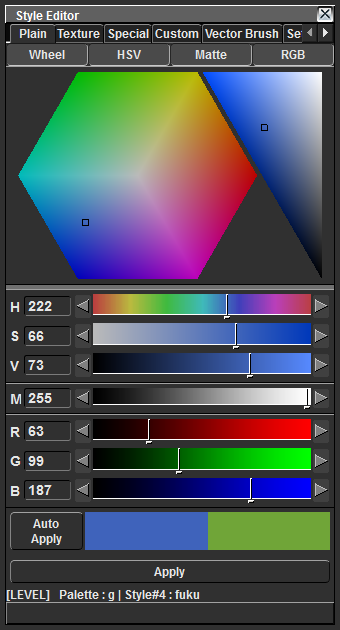
\includegraphics[width=14.5em]{PaletteStyleEditingStyleEditor}}
\color{white}
\put(13,144){●}
\put(13,132){●}
\put(35,112){●}
\put(9.5,-12){\normalsize{●}}
\put(9.5,-43){\normalsize{●}}
\put(9.5,-75){\normalsize{●}}
\put(62,-108.5){●}
\put(20,-112){●}
\color{red}
\put(13,144){①}
\put(13,132){②}
\put(35,112){③}
\put(9.5,-12){\normalsize{④}}
\put(9.5,-43){\normalsize{⑤}}
\put(9.5,-75){\normalsize{⑥}}
\put(62,-108.5){⑦}
\put(20,-112){⑧}
\end{picture}\\[12.2em]

\normalsize
\noindent Palette Gizmo… For the selected style, this window is used for the color operations.\\[-0.5em]

\large
\noindent\begin{picture}(0,0)
\put(3,-125){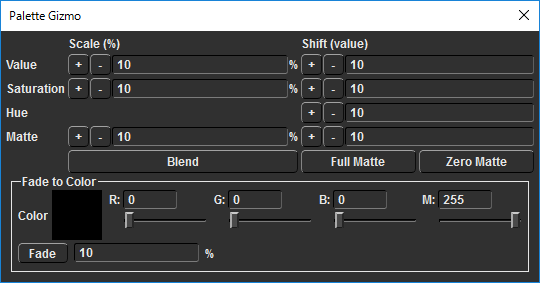
\includegraphics[width=20em]{PaletteStyleEditingPaletteGizmo}}
\color{white}
\put(-6,-31.5){\normalsize{●}}
\put(21,-23){●}
\put(125,-23){●}
\put(63,-76){●}
\put(137.5,-76){●}
\put(189,-76){●}
\put(0,-85){●}
\color{red}
\put(-6,-31.5){\normalsize{①}}
\put(21,-23){②}
\put(125,-23){③}
\put(63,-76){④}
\put(137.5,-76){⑤}
\put(189,-76){⑥}
\put(0,-85){⑦}
\end{picture}\\[-3.2em]

\footnotesize
\noindent \hskip 31.25em ① Value (Brightness), Saturation, Hue, Matte\par
\noindent \hskip 31.25em ② [Scale(\%)]: [+][-] Percentage amount of current value.\par
\noindent \hskip 31.25em ③ [Shift(value)]: Numerical amount from current value.\par
\noindent \hskip 31.25em ④ [Blend]: Only valid when selecting more than 3 styles.\par
\noindent \hskip 31.25em Automatically blends the first \& last style colors.\par
\noindent \hskip 31.25em ⑤ [Full Matte]: All Matte values of the selected style\par
\noindent \hskip 31.25em will become 255.\par
\noindent \hskip 31.25em ⑥ [Zero Matte]: All Matte values of the selected style\par
\noindent \hskip 31.25em will become 0.\par
\noindent \hskip 31.25em ⑦ [Fade To Color]: Set Color RGBM values \& press the\par
\noindent \hskip 31.25em Fade button, colors values will be set to the \% amount.

\newpage

\normalsize
\noindent Palette… Palette tool that shows the contents of the tpl file that that is linked with the tlv.

\large
\noindent\begin{picture}(0,0)
\put(3,-75){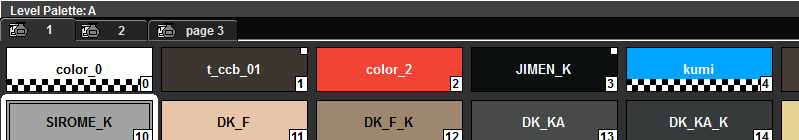
\includegraphics[width=39em]{PaletteStyleEditingLevelPalette}}
\color{white}
\put(52,6){\normalsize{●}}
\put(9,-15){●}
\put(116,-38.5){●}
\put(373.5,-38.5){●}
\put(174,-39){●}
\color{red}
\put(52,6){\normalsize{①}}
\put(9,-15){②}
\put(10,-31){\normalsize{③}}
\put(116,-38.5){④}
\put(373.5,-38.5){⑤}
\put(174,-39){⑥}
\end{picture}\\[4.9em]

\footnotesize
\noindent ① Palette Name\\
② Page: You can save to add \& delete palettes on the page, using the right-click menu. It is switched using the tab.\\
③ Style: You will see a white frame in the style of the selection. Select a style, you can move using ctrl key + drag.\\
④ Style-Name: Double-click to change the name.\\
⑤ Matte value, shown at the bottom as a checkered display. Checker will appear darker when the value is smaller.\\
⑥ Style Number: If you change the arrangement of the style, this number will not change.

\large
\noindent\begin{picture}(0,0)
\put(3,-115){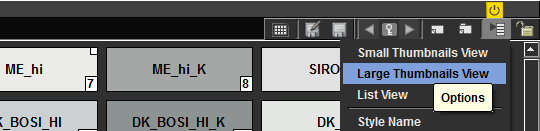
\includegraphics[width=39em]{PaletteStyleEditingViewOptions}}
\color{white}
\put(240,-20){●}
\put(268,-20){●}
\put(291,-20){●}
\put(334,-20){●}
\put(376,-20){●}
\put(401,-20){●}
\put(423.5,-30.5){●}
\put(454.5,-20){●}
\color{red}
\put(240,-20){①}
\put(268,-20){②}
\put(291,-20){③}
\put(334,-20){④}
\put(376,-20){⑤}
\put(401,-20){⑥}
\put(423.5,-30.5){⑦}
\put(454.5,-20){⑧}
\end{picture}\\[8.3em]

\footnotesize
\noindent ① [Palette]: By Drag-\&-Drop into the Studio Palette, adds it as a new page of the Current Palette to Studio Palette.\\
② [Save Palette As]: Saves the Current Palette with a filename alias.\\
③ [Save Palette]: Saves the Current Palette.\\
④ [Set Key]: By setting the key color chip, you can create more than 1 color in the tpl file.\\
⑤ [New Style]: Used to add a style.\\
⑥ [New Page]: Used to add a page to the palette.\\
⑦ The display switching menu of the palette.\\
⑧ [Lock Palette]: You can toggle whether the editing of the palette content is locked/unlocked.\\

\phantomsection
\subsection*{\uline{□ Studio Palette Information}}
\addcontentsline{toc}{subsection}{□ Studio Palette Information}

\normalsize
\noindent Studio Palette… This window is used to display a palette that will become a color swatch.\\

\phantomsection
\subsection*{\uline{□ Studio Palette Folder Creation \& Deletion, to Create a New Palette.}}
\addcontentsline{toc}{subsection}{□ Studio Palette Folder Creation \& Deletion, to Create a New Palette.}

\vspace{1.5em}

\noindent \hskip 17em Toonz Palettes… Specifies the \small\$TOONZSTUDIOPALETTES \normalsize folder\par
\noindent \hskip 17em (usually studiopalettes inside Stuff folder) shows contents.\par
\noindent \hskip 17em Project Palettes… +palettes project folder will be displayed.\\
\par
\footnotesize
\noindent \hskip 21.25em ※ Toonz Palette to be used by the whole studio, Project Palette is the palette\par
\noindent \hskip 21.25em  to be used for all the work.

\large
\noindent\begin{picture}(0,0)
\put(7,-69){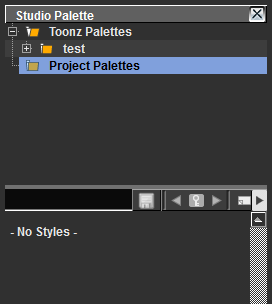
\includegraphics[width=12.9em]{StudioPaletteProjectPalettes}}
\linethickness{0.1em}
\color{red}
\put(165,100){\line(-5,-1){75}}
\put(165,67){\line(-1,0){75}}
\end{picture}

\newpage

\large
\noindent\begin{picture}(0,0)
\put(15,-177){\includegraphics[width=12.4em]{StudioPaletteNewPalette}}
\linethickness{0.1em}
\color{red}
\put(170,-35){\line(-6,1){66}}
\end{picture}\\[0.3em]

\footnotesize
\noindent \hskip 22em New Palette… Creates a new Palette.\par
\noindent \hskip 22em New Folder… Creates a new folder.\par
\noindent \hskip 22em Delete Folder… Deletes the folder. Palettes in the folder are also deleted.\par
\noindent \hskip 22em Search for Palette… Allows you to search for a specific palette.\\[10.5em]

\noindent \,Studio Palette style that was copied from the style that was saved, you can copy the original style \& links.\\
・Link a style \& it will be marked with a rectangle in the upper right corner. When the color of the link style changes\\
from the color that has been registered in the Studio Palette, it will be displayed hatched.\\
・Select a style, selected by the [Right-Click Menu/Get Color from Studio Palette], to return to the registered link\\
 source of the Studio Palette style color.\par
\noindent \hskip 27em ・To remove a link, select the [Right-Click Menu/Remove Links],\par
\noindent \hskip 27em \ \& choose a link, \& it will remove the link from the Studio Palette.

\large
\noindent\begin{picture}(0,0)
\put(3,-44){\includegraphics[width=17.4em]{StudioPaletteRemoveLinks}}
\end{picture}

\newpage

\phantomsection
\subsection*{\uline{□ Viewing the Image (Windows/)}}
\addcontentsline{toc}{subsection}{□ Viewing the Image (Windows/)}

\normalsize
\noindent Combo Viewer… This window is used to display the image.\par
\footnotesize
\noindent Using the right-click menu on the window, various functions are available, to modify the display.\\
\par
\noindent \uline{【View Mode Menu】}\\
① [Camera Stand View]: Used to view the original size of the image. You typically select work in here.\\
② [3D View]: It displays the positional relationship between the camera \& the image material in 3D.\\
③ [Freeze]: In Preview display mode, even if there is a change to the image, it will not update the Preview display.\\
④ [Preview]: Camera Size is set in the Output Settings, \& the  image will display including any applied effects.

\large
\noindent\begin{picture}(0,0)
\put(279,-34){\includegraphics[width=13.7em]{ViewingTheImageViewModeMenu}}
\put(104,-232){\includegraphics[width=22.4em]{ViewingTheImageViewer}}
\put(3,-280){\includegraphics[width=39em]{ViewingTheImageConsoleMenu}}
\linethickness{0.1em}
\color{red}
\put(346.5,7){\normalsize{①}}
\put(356.5,7){\normalsize{②}}
\put(379.5,7){\normalsize{③}}
\put(393,7){\normalsize{④}}
\put(4.5,-251){\normalsize{①}}
\put(22.5,-251){\normalsize{②}}
\put(40.5,-251){\normalsize{③}}
\put(57.5,-251){\normalsize{④}}
\put(96.5,-251){\normalsize{⑤}}
\put(114.5,-251){\normalsize{⑥}}
\put(131.5,-251){\normalsize{⑦}}
\put(152,-251){\normalsize{⑧}}
\put(169,-251){\normalsize{⑨}}
\put(185.5,-251){\normalsize{⑩}}
\put(202,-251){\normalsize{⑪}}
\put(220,-251){\normalsize{⑫}}
\put(237,-251){\normalsize{⑬}}
\put(256,-251){\normalsize{⑭}}
\put(290,-251){\normalsize{⑮}}
\put(328,-251){\normalsize{⑯}}
\put(357,-251){\normalsize{⑰}}
\put(423.5,-251){\normalsize{⑱}}
\put(275,05){\line(1,0){166}}
\put(275.5,05){\line(0,-1){39}}
\put(440.5,05){\line(0,-1){39}}
\put(275,-34){\line(1,0){166}}
\put(344,-34){\line(-1,-4){3.7}}
\put(183,-254){\line(-1,6){4.6}}
\put(0,-254){\line(1,0){469}}
\put(0,-254){\line(0,-1){26}}
\put(468.4,-254){\line(0,-1){26}}
\put(0,-280){\line(1,0){469}}
\end{picture}\\[22.8em]

\footnotesize
\noindent \uline{【Console Menu】}\\
① Show/Hide options\\
② Save image that is displayed in a format that you have set in the Output Settings. Only Preview mode is enabled.\\
③ Stores one frame of the image displayed on the memory. This feature is used in ④.\\
④ The frame that is stored with “③", is compared with the display of the frame you are currently previewing.\\
⑤ Display the background color using RGB set to 255\\
⑥ Display the background color using RGB set to 0\\
⑦ Display the background color using Matte set to 0\\
⑧ Move to the first frame\\
⑨ Step Back 1 frame\\
⑩ Pause the frame\\
⑪ Play frames\\
⑫ Loop playback of frames\\
⑬ Step Forwards 1 frame\\
⑭ Move to the last frame\\
⑮ A button selection for each of the R,G,B, \& Matte, for the image color information when you click the Display\\
⑯ Display a histogram of the image\\
⑰ Set the key frame. Go to the key frame using the left \& right buttons.\\
⑱ Specifies the frame rate during playback.

\newpage

\phantomsection
\subsection*{\uline{□ Time Sheet Editing (Windows/)}}
\addcontentsline{toc}{subsection}{□ Time Sheet Editing (Windows/)}

\normalsize
\noindent Xsheet… Place image files, such as tlv or tif, it has a window for each work segment.\par
\footnotesize
\noindent Cell Stacking order goes from left to right, the top \& bottom displays the time axis.\\
\par
\noindent \hskip 22.5em ① Show/Hide during preview\par
\noindent \hskip 22.5em ② Camera Stand Show/Hide\par
\noindent \hskip 22.5em ③ Thumbnail displays the first frame of the column\par
\noindent \hskip 22.5em ④ Displays the Table type\par
\noindent \hskip 22.5em ⑤ Displays the Column・Cells

\large
\noindent\begin{picture}(0,0)
\put(7,-82){\includegraphics[width=13.4em]{TimeSheetEditingXsheet}}
\color{white}
\put(64,63.5){●}
\put(64,51.5){●}
\put(64,33.5){●}
\put(64,16.4){●}
\put(64,-23){●}
\color{red}
\put(64,63.5){①}
\put(64,51.5){②}
\put(64,33.5){③}
\put(64,16.4){④}
\put(64,-23){⑤}
\end{picture}\\[6em]

\footnotesize
\noindent \uline{【Right-Click Menu】}\\
※ The following items will be applied to Cells you have selected.\\
\ [Step]: Changes the frame step. Example) Step2 = 2 frames beating\\
\ [Each]: Thins out the cut amount. Example) Each2 1,2,3,4,5 → 1,3,5\\
\ [Reverse]: Reverse the content order.\\
\ [Swing]: Reverse content is added to the content.\\
\ [Random]: Sort randomly.\\
\ [Repeat]: Sets content repetition copy.\\
\ [Roll Up]: Move content up 1 frame.\\
\ [Roll Down]: Move content down 1 frame.\\
\ [Time Stretch]: Numerically Time Stretch content.\\
\\
\ [Replace Level]: Load new material over current Cells.\\
\ [Revert to Cleaned Up]: Replace selected Cells with No paint data.\\
\ [Info]: Displays the information from the selected image.\\
\ [View]: Displays the selected image.

\large
\noindent\begin{picture}(0,0)
\put(273,-5){\includegraphics[width=16.6em]{TimeSheetEditingRightClickMenu}}
\end{picture}\\[-1.2em]

\phantomsection
\subsection*{\uline{□ Viewing the Color Swatch Used in Painting (Windows/)}}
\addcontentsline{toc}{subsection}{□ Viewing the Color Swatch Used in Painting (Windows/)}

\normalsize
\noindent Color Model… Color sample a tlv image at the time of paint \& then Load. This window can be used\\
to extract color from an image.\\[-0.5em]
\par
\footnotesize
\noindent \uline{【Right-Click Menu】}\\
\ [Load Color Model]: Browser to select the tlv will be displayed. Select the file to read the Color Model.\\
※ If you Load a tlv with multiple frames, you can move the frame in the Console. The Warning window will display, choose\\
one of the options.\\
・Overwrite the destination palette… The tpl of the selected color model, overwrites to the currently selected tlv color\\
model. (tlv as a sample) will be replaced by the color of the color model Load.\\
・Keep the destination palette and apply it to the color model… tpl of the selected color model will not Load. Pixels\\
will use tpl data from current work. It will remain to be used. Load color model with the color from the current work.\\
\\
\ [Use Current Frame]: Load the currently selected tlv frame as the Color Model.\\
\ [Remove Color Model]: Clears the Color Model.\\
※ Reading from a tga format image file, it is also possible to extract the RGB values from the image.

\newpage

\phantomsection
\subsection*{\uline{□ Browsing the Files (Windows/)}}
\addcontentsline{toc}{subsection}{□ Browsing the Files (Windows/)}

\normalsize
\noindent File Browser… This window is used to browse the files.\par
\footnotesize
\noindent Please see more information about this window, in “File Browser Interface" (p.4).\\
You can not Load files in this window. Creating a directory, \& the display of file information is available.\\

\phantomsection
\subsection*{\uline{□ tlv Frame Viewing (Windows/)}}
\addcontentsline{toc}{subsection}{□ tlv Frame Viewing (Windows/)}

\normalsize
\noindent Level Strip… Displays the frames of a tlv file, it has a window that you can edit from.\\
\par
\footnotesize
\noindent \hskip 21.25em ① Selects a tlv that will Load in the Scene. Files that are displayed with\par
\noindent \hskip 21.25em “*" are in a state where the changes have not yet been saved.\par
\noindent \hskip 21.25em ② Frame Number\par
\noindent \hskip 21.25em ③ Currently selected frame with a red border is displayed on the Viewer.\par
\noindent \hskip 21.25em You can change the position of the View Range when you drag on the frame.\par
\noindent \hskip 21.25em In addition the edited image, will be updated in real-time on the display.\\
\par
\noindent \hskip 21.25em 【Right-Click Menu】\par
\noindent \hskip 21.25em [Select All]: Select all of the frames.\par
\noindent \hskip 21.25em [Invert Selection]: All the selected frames will be inverted.\par
\noindent \hskip 21.25em [Cut]: Cuts the selected frame.\par
\noindent \hskip 21.25em [Copy]: Copies the selected frame.\par
\noindent \hskip 21.25em [Insert Paste]: Insert material stored using Copy into the selected frame.\par
\noindent \hskip 21.25em [Paste Into]: Copy frames, \& paste into selected frames.\par
\noindent \hskip 21.25em [Merge]: Copy a frame, \& paste it to the location that corresponds to the\par
\noindent \hskip 21.25em frame number of the currently selected tlv.\par
\noindent \hskip 21.25em [Insert]: Select  (from) the number of frames, to insert empty frames.\par
\noindent \hskip 21.25em [Delete]: Clears the image of the selected frame. Frame will not be erased.\par
\noindent \hskip 21.25em [Duplicate Drawing]: Select frames, copy \& pastes to the bottom of the frames.\par
\noindent \hskip 21.25em [Reverse]: Reverses of the order of selected frames. Example) 1,2,3 → 3,2,1\par
\noindent \hskip 21.25em [Swing]: Adds reversed selected frames. Example) 1,2,3,4 → 1,2,3,4,3,2,1\par
\noindent \hskip 21.25em [Step2~4]: Increase selected frames time. Example) Step2 1,2,3 → 1,1,2,2,3,3\par
\noindent \hskip 21.25em [Each2~4]: Cut the selected frames time. Example) Each2 1,2,3,4 → 1,3\par
\noindent \hskip 21.25em [Expose in Xsheet]: Adds the selected frame to the Xsheet.\par
\noindent \hskip 21.25em [Add Frames]: Dedicated window is displayed, with a numeric input to add a\par
\noindent \hskip 21.25em  nunber of empty frames that will be inserted (from).\par
\noindent \hskip 21.25em [Renumber]: Changes the frame number of the selected frames.\par
\noindent \hskip 21.25em [Revert to Cleaned Up]: Overwrite the selected frame with data in No paint.\par
\noindent \hskip 21.25em Cleanup image will return immediately afterwards.

\large
\noindent\begin{picture}(0,0)
\put(3,30){\includegraphics[width=13.4em]{TLVFrameViewingLevelStrip}}
\color{white}
\put(41,367){●}
\put(94,279){●}
\color{red}
\put(41,367){①}
\put(94,279){②}
\put(52,306){\normalsize{③}}
\end{picture}\\[0.5em]

\normalsize
\noindent Toolbar… This window is used to display the various Tools.\par
\footnotesize
\noindent Please refer to the “Tools" (p.13~) for information about each function.\\[-0.5em]
\par
\normalsize
\noindent Tool Option Bar… This window is used to display the Tool Option Bar.\par
\footnotesize
\noindent Please refer to the description of each Tool to learn more about the functions.\\[-0.5em]
\par
\normalsize
\noindent Reset to Default Rooms… Used to reset the configuration of the room to the initial state.\\[-0.5em]
\\
Batch Servers… Used to set whether to perform Batch calculations on any machines.

\newpage

\phantomsection
\subsection*{\uline{□ Previewing Image Sequences in a Video (Windows/)}}
\addcontentsline{toc}{subsection}{□ Previewing Image Sequences in a Video (Windows/)}

\normalsize
\noindent Flipbook… Plays the video, it has a window if you want to save.\par
\footnotesize
\noindent Load tif \& tlv rgb image files, to be animated.\\
\par
\normalsize
\noindent Also in the Console Menu of the Viewer, you can play an image sequence that will display as a video.\\
\\
Function Editor… Xsheet camera column, has a window that can be set by numerical input.\\[1em]
Scene Cast… A window that displays the image Load file that is currently being sent to the Scene.\par
\footnotesize
\noindent Even if the files are hidden on the Xsheet, Load files will be displayed in the Scene Cast.\\
※ Files to be remove from the cell in the Xsheet are registered in the Scene Cast as a state of being Loaded.\\
To cancel the registration of the file, select the Cast file, \& run the Right-Click Menu / [Remove Level].\\
\par
\normalsize
\noindent Schematic… Xsheet Camera material, has a window that can display a status effects flow chart.\\
\\
Tasks… This window is used to display the Task Batches.\par
\footnotesize
\noindent Load a tnz file to do batch processing.\\
\\

\phantomsection
\subsection*{\uline{□ Environment Settings \& Keyboard Shortcuts (Customize/)}}
\addcontentsline{toc}{subsection}{□ Environment Settings \& Keyboard Shortcuts (Customize/)}

\normalsize
\noindent Preferences… This is a menu for all of the environment settings in Toonz.\\
\\
Configure Shortcuts… This menu is used for setting the keyboard shortcuts in Toonz.\\
\\
Scene Settings… This menu has settings such as the background color \& the camera Frame rate.\\

\phantomsection
\subsection*{\uline{□ Various Display Menus (Customize/)}}
\addcontentsline{toc}{subsection}{□ Various Display Menus (Customize/)}

\normalsize
\noindent View… Contains various menus to change the display in the Combo Viewer.\par
\footnotesize
\noindent [Camera Box]: The camera size set in Output Settings, will be displayed as a red dashed line on the Viewer. * It does\\
not appear when the tlv file has been selected in the InknPaint Room.\\
\ [Table]: Displays the Camera Stand in the background.\\
\ [Field Guide]: This is a grid-shaped guide display. Units are in inches.\\
\ [Safe Area]: At the time of Camera Box display, it displays the actual area that will be shown on the television screen.\\
\ [Camera BG Color]: Displays the background below the image file. Size is the camera size set in Output Settings.\\

\phantomsection
\subsection*{\uline{□ Window Layout Customization (Customize/)}}
\addcontentsline{toc}{subsection}{□ Window Layout Customization (Customize/)}

\normalsize
\noindent Lock Room Panes… Switch menu to Lock/Unlock the current windows layout in a Room.

\newpage

\phantomsection
\subsection*{\uline{□ tlv File Conversion to Other File Formats}}
\addcontentsline{toc}{subsection}{□ tlv File Conversion to Other File Formats}

\footnotesize
\noindent Finishing work files in OpenToonz, \& for saving a file to be used in other software, you will need to do the conversion\\
(Export) of the file to a new format.\\[-0.5em]
\par
\normalsize
\noindent 1. Right-Click on the file you want to convert in the File Browser \& select [Convert].

\large
\noindent\begin{picture}(0,0)
\put(117,-153){\includegraphics[width=19.2em]{TLVFileConversionToOtherFileFormats}}
\color{white}
\put(132.5,-92){\small{●}}
\put(132.5,-101){\small{●}}
\color{red}
\put(108,-44){\footnotesize{①}}
\put(108,-52.5){\footnotesize{②}}
\put(108,-61){\footnotesize{③}}
\put(108,-69.5){\footnotesize{④}}
\put(108,-82){\footnotesize{⑤}}
\put(132.5,-92){\small{⑥}}
\put(132.5,-101){\small{⑦}}
\end{picture}\\[11.75em]

\footnotesize
\noindent ① Enter the frame range that you want to create.\\
② Choose a location for the file to be created.\\
③ Enter the file name.\\
④ Select the file format.\\
⑤ Set the background color. This is usually RGB all 255 (White).\\
⑥ When checked, if you have the same file in the destination, creates only new files without overwriting existing files.\\
⑦ When checked, it removes the [.(Dot)] attached to the front of the frame number of the tlv file name before conversion.\\
Example) File Name is “A" \ Remove dot before the frame number in the case of “OFF": A.0001.tga, A.0002.tga, A.0003.tga...\\
Example) File Name is “A\_" Remove dot before the frame number in the case of “ON": A\_0001.tga, A\_0002.tga, A\_0003.tga...\\
※ Only if the file format after the conversion is not selected to be a tlv, will this function be enabled.\\
※ OpenToonz filename form, is between the level name \& the last four digits of the frame number “." (Dot) or\\
“\_" (Underscore), it can then be recognized as  a series of frames in the Level.\\
\par
\normalsize
\noindent 2. When you click the [Convert] button, it will start to Convert the frames.

\newpage

\phantomsection
\section*{\uline{■ PltEdit}}
\addcontentsline{toc}{section}{■ PltEdit}

\footnotesize
\noindent In PltEdit Room, you can create files with extensive background material \& cells, \& edit the palettes. Among the finishing\\
process, \& mainly used in the scene to determine the color.\\

\phantomsection
\subsection*{\uline{□ Sheet Creation to Perform Color Designation}}
\addcontentsline{toc}{subsection}{□ Sheet Creation to Perform Color Designation}

\footnotesize
\noindent In determining the colors, you can create a sheet of the required files.\\
\par
\normalsize
\noindent 1. BG (Background Material) files \& painted tlv files to read into the sheet.\par
\footnotesize
\noindent Select the column that you want side-by-side on the Xsheet, read the tlv files into the Load Level.\\
Read the BG into column 1 of the Xsheet (Material will becomes the furthest-back). Other Book materials \& each cell will\\
read the file in the actual stacking order of the time sheet. Also will read the files of the layout for the alignment.\\
\par
\normalsize
\noindent 2. Moves to match the position of BG with the position of the layout file.\par
\footnotesize
\noindent If the BG is shifted to the layout, it will do the alignment.\\
It shows only the layout \& the BG.\\
Select the file (BG) that you want to move, \& it will be moved according to the layout using the Edit Tool.\\
※ Layout files, do not require the cell to be displayed in the preview all the time, you can switch the cells\\
Display/Non-Display by clicking the [Preview Visibility Toggle] at the top of each cell on the Xsheet.\\
\par
\normalsize
\noindent 3. If there is a Book, move the position as well as the BG.\par
\footnotesize
\noindent Select the [Windows/Other Windows/Schematic], to display the Schematic window.\\
To align the Book as a member of column 1 (BG), on the Stage Schematic, click \& drag the Blue ● of the Book, connect\\
it to the Red ● of column 1.\\
※ If the white edge of the Book at the time of the preview is displayed to select the Book on the FX Schematic, and then\\
select the [Right-Click Menu /Insert FX/Layer Blending/Premultiply]. Also by putting a check in the [Premultiply] of\\
Select the Book Level Settings, you can turn off the edge at the time of preview.\\
\par
\normalsize
\noindent 4. Use the Style Editor \& Studio Palette to edit the style.\par
\footnotesize
\noindent You can also extract the color from the background image using the RGB Picker Tool.\\
Run the preview, it is also possible to check the screen state multiplied by the processing.\\
\\

\phantomsection
\subsection*{\uline{□ Displaying a Specific Frame}}
\addcontentsline{toc}{subsection}{□ Displaying a Specific Frame}

\normalsize
\noindent You can arrange only the necessary frame number in the Xsheet, or using the Sub-Xsheet, it is\\
 also possible to preview only the sheet number required.\\
\par
\noindent 【How to Create a Sub-Xsheet】\\
Select the cell you want to include, \& then select the [Right-Click Menu /Collapse]. The following\\
alert window is displayed.\par
\footnotesize
\noindent ・Include relevant pegbars in the sub-xsheet as well…  Information of the Pegbar is also included in the Sub-Xsheet.\\
・Include only selected columns in the sub-xsheet… Information of the Pegbar is not included in the Sub-Xsheet.\\
Sub-Xsheet appears as purple on the Xsheet.\\
When you are folding the data into the Sub-Xsheet, you implant the sheet number you want to preview.

\newpage

\phantomsection
\subsection*{\uline{□ Previewing in a Transparent Display}}
\addcontentsline{toc}{subsection}{□ Previewing in a Transparent Display}

\footnotesize
\noindent Add the effects in a simple manner on the Schematic.\\[-0.5em]
\par
\small
\noindent 1. Copy the cell which you want to apply the processing. Arrange 2 of the same cell on the Xsheet.\\
\\
2. In Fx Schematic, select each cell, \& use [Right-Click Menu /Insert FX/Toonz Level/Palette Filter].\\
Once the FX has been added, Double-Click the FX. A setup screen will appear.\\
\par
\footnotesize
\noindent \hskip 30.25em [Color Indexes]: Enter the double cell sheet style number.\par
\noindent \hskip 30.25em [Action]: Select keep on 1 cell, on the other cell select\par
\noindent \hskip 30.25em Delete.

\large
\noindent\begin{picture}(0,0)
\put(3,-120){\includegraphics[width=19.3em]{PreviewingTransparentDisplayFxSchematic}}
\end{picture}\\[9.25em]

\small
\noindent Select the FX of the cell which was selected to Keep the\\
Action of the item, then select [Right-Click Menu /Insert FX\\
/Layer\_Blending/Transparency]. You can also change settings\\
of the strength of the treatment with a Double-Click.\par
\footnotesize
\noindent When previewed, it will display the double brush processing result.\\
On the display, the double cell is overlaped with the shadow of the\\
other cell. The cell for double brush shadow that you copied to the\\
Sub-Xsheet, is multiplied by Transparency processing, a shadow is\\
made from the 2 cells, tweak the transparency to suit your needs.

\large
\noindent\begin{picture}(0,0)
\put(271,-4){\includegraphics[width=16.8em]{PreviewingTransparentDisplayTransparency}}
\end{picture}

\end{document}